\documentclass[
	aps, pra, authorblock, superscriptaddress, twocolumn,
	10pt
]{revtex4-1}
\usepackage[final]{graphicx}
\graphicspath{{./figures/}}
\usepackage{times,bbm,amsmath,amssymb}
\usepackage{microtype}
\usepackage{epsfig,color}
\usepackage{xcolor}
\usepackage{hyperref}
\hypersetup{
    colorlinks = true
}
\usepackage{cleveref}

\usepackage{libertine}

\usepackage{float,siunitx}
\usepackage[caption = false]{subfig}

\usepackage[greek,english]{babel}
% \usepackage{thumbpdf,enumerate}
\usepackage{booktabs}
% \usepackage{sidecap}
% \usepackage[scaled=.8]{couriers}    
% \usepackage{pstricks}
\usepackage{multirow}
\usepackage{placeins}
\usepackage{relsize}  
% \usepackage{pst-grad,bm}
% \usepackage{epigraph}
% \usepackage{gensymb}
% \usepackage{longtable}
% \usepackage{booktabs}
% \usepackage{gensymb}

% \usepackage{soul}
% \usepackage{ulem}
% \normalem 

\usepackage{acronym}
% \usepackage{todonotes}
\usepackage{easyReview}

\usepackage{tikz}
\usetikzlibrary{quantikz}
\usepackage{physics}

\newcommand{\bs}[1]{\boldsymbol{#1}}
\newcommand{\on}[1]{\operatorname{#1}}
\newcommand{\U}{\mathcal{U}}
\newcommand{\CC}{\mathbb{C}}
\newcommand{\PP}{\mathbb{P}}
\newcommand{\RR}{\mathbb{R}}
\newcommand{\ZZ}{\mathbb{Z}}

\newcommand{\calE}{{\mathcal{E}}}
\newcommand{\calH}{{\mathcal{H}}}
\newcommand{\calU}{{\mathcal{U}}}
\newcommand{\calV}{{\mathcal{V}}}


\begin{document}
\title{Quantum walks with entangled qubits: notes for Rome} 
\author{Belfast, August 2019}
\maketitle

In these notes we report the preliminary results about the problem of two 
local quantum walks routine, starting from two entangled qubits. The first question we want to address concern the possibility to transfer the \emph{ebit} of entanglement in the coin degree of freedom, i.e. the amount of entanglement contained in a Bell state, to the the bipartite system made by the position of the two resulting walkers. In our setup for QWs, that encode the evolution in the angular momentum degree of freedom \cite{giordani_2018}, this means to convert the entanglement in polarization to a state of two entangled qudit in the orbital angular momentum (see \Cref{fig:concept}).

These notes are organised as follows: in the first section we state the formalism of the problem; in the second we investigate the amount of residual correlation between the two parties in the position spaces when the coin is traced out. In the third part we focus on joint walkers states after proper projection of the two coin. We found that is always possible to recover the ebit of entanglement for a suitable coin-measurement choice. In the fourth section we discuss a protocol for entanglement accumulation and a possible experimental implementation. Then, we conclude with the open problem that we are discussing in Belfast.
\section{Problem statement}
Let us introduce some useful notation that we will use throughout the notes. In our problem we have to deal with a four-partite system, namely coin and position for the first particle, labelled as $(c_1, \, w_1)$, and for the second particle $(c_2, \, w_2)$. The subsystems $c_i$ are two dimensional, while the position space $w_i$ is $(N_{i}+1)$-dimensional, where $N_{i}$ is the number of steps of the QW.
The input state produced by the source can expressed as follows:
\begin{equation}
    \ket{\Psi^0} = \frac{1}{\sqrt{2}}
    \left ( \ket{\uparrow}_{c_1}\ket{\downarrow}_{c_2}+ \mathrm{e}^{\mathrm{i}\phi}\ket{\downarrow}_{c_1}\ket{\uparrow}_{c_2}\right ) \otimes \ket{0}_{w_1}\ket{0}_{w_2} 
    \label{eq:initial_state}
\end{equation}
where we refer to $k=\{\ket{\uparrow}, \ket{\downarrow}\}$ as the coin basis and the states $\ket{s}$, with $s=\{-(2N+1),..., 2N+1\}$ as the walker position. The resulting state after the two quantum walks will be $\ket{\Psi^f}=U_{c_1,w_1} \otimes U_{c_2,w_2},  \ket{\Psi^0}$, in which the two local unitaries are made by the combination of coin and shift operator of the quantum walk evolution. Then given the structure of the input state, the expression for the final state will be in the following form
\begin{equation}
\ket{\Psi^f} = \alpha \ket{\Psi^{\uparrow}_1\Psi^{\downarrow}_2 }+\beta \ket{\Psi^{\downarrow}_1\Psi^{\uparrow}_2},
\label{eq:final_state}
\end{equation}
where each single particle state $\ket{\Psi^k_i}$ refers to the output of a single particle QW $U_{c_i,w_i}$, with $k$ as input state.

A common criterion for discerning if a multipartite state is separable or not, is the PPT criterion (positivity of the partial tranpose) \cite{HORODECKI19961}. Such method envisage the calculation of eigenvalues of the partial transpose respect with one subsystem of the density matrix representing the entire system. If there exists at least one non-positive eigenvalue the state cannot be separable. This criterion is a sufficient condition of non-seprability of the multipartite state. Furthermore we can provide an estimation of the amount of entanglement through the state \emph{negativity} $\mathcal{N}$, i.e the sum of the negative eigenvalues of the partial transpose density matrix. The initial state in the joint coin subspaces has $\mathcal{N}^{Bell}=\frac{1}{2}$, namely a one ebit of entanglement. In this notes we will consider the negativity of the states normalized to one ebit, i.e $\mathcal{N}/\mathcal{N}^{Bell}.$


\begin{figure}[b]
    \centering
    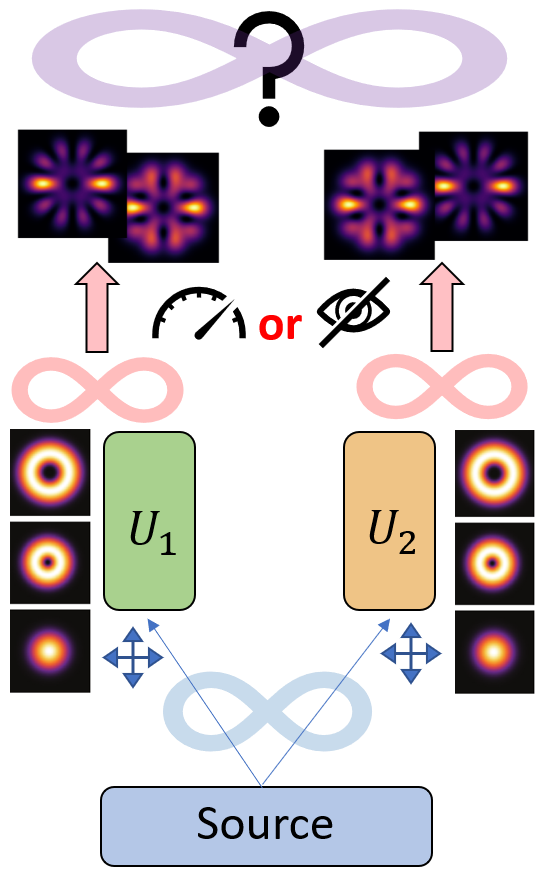
\includegraphics[scale=0.35]{concept.png}
    \caption{\textbf{Scheme of the problem.} The Bell state produced by a single-photon source represents the entangled input state for the two independent quantum walks. The latter evolution enlarge the space of each subsystem, creating correlation between the polarization (the coin) and orbital angular momentum (walker position). We ask for the amount of entanglement in the walkers space after \textit{i)} tracing the polarization or \textit{ii)} projecting the coins. }
    \label{fig:concept}
\end{figure}

\section{Tracing out different subsystems}

 \begin{figure*}[t]
    \centering
    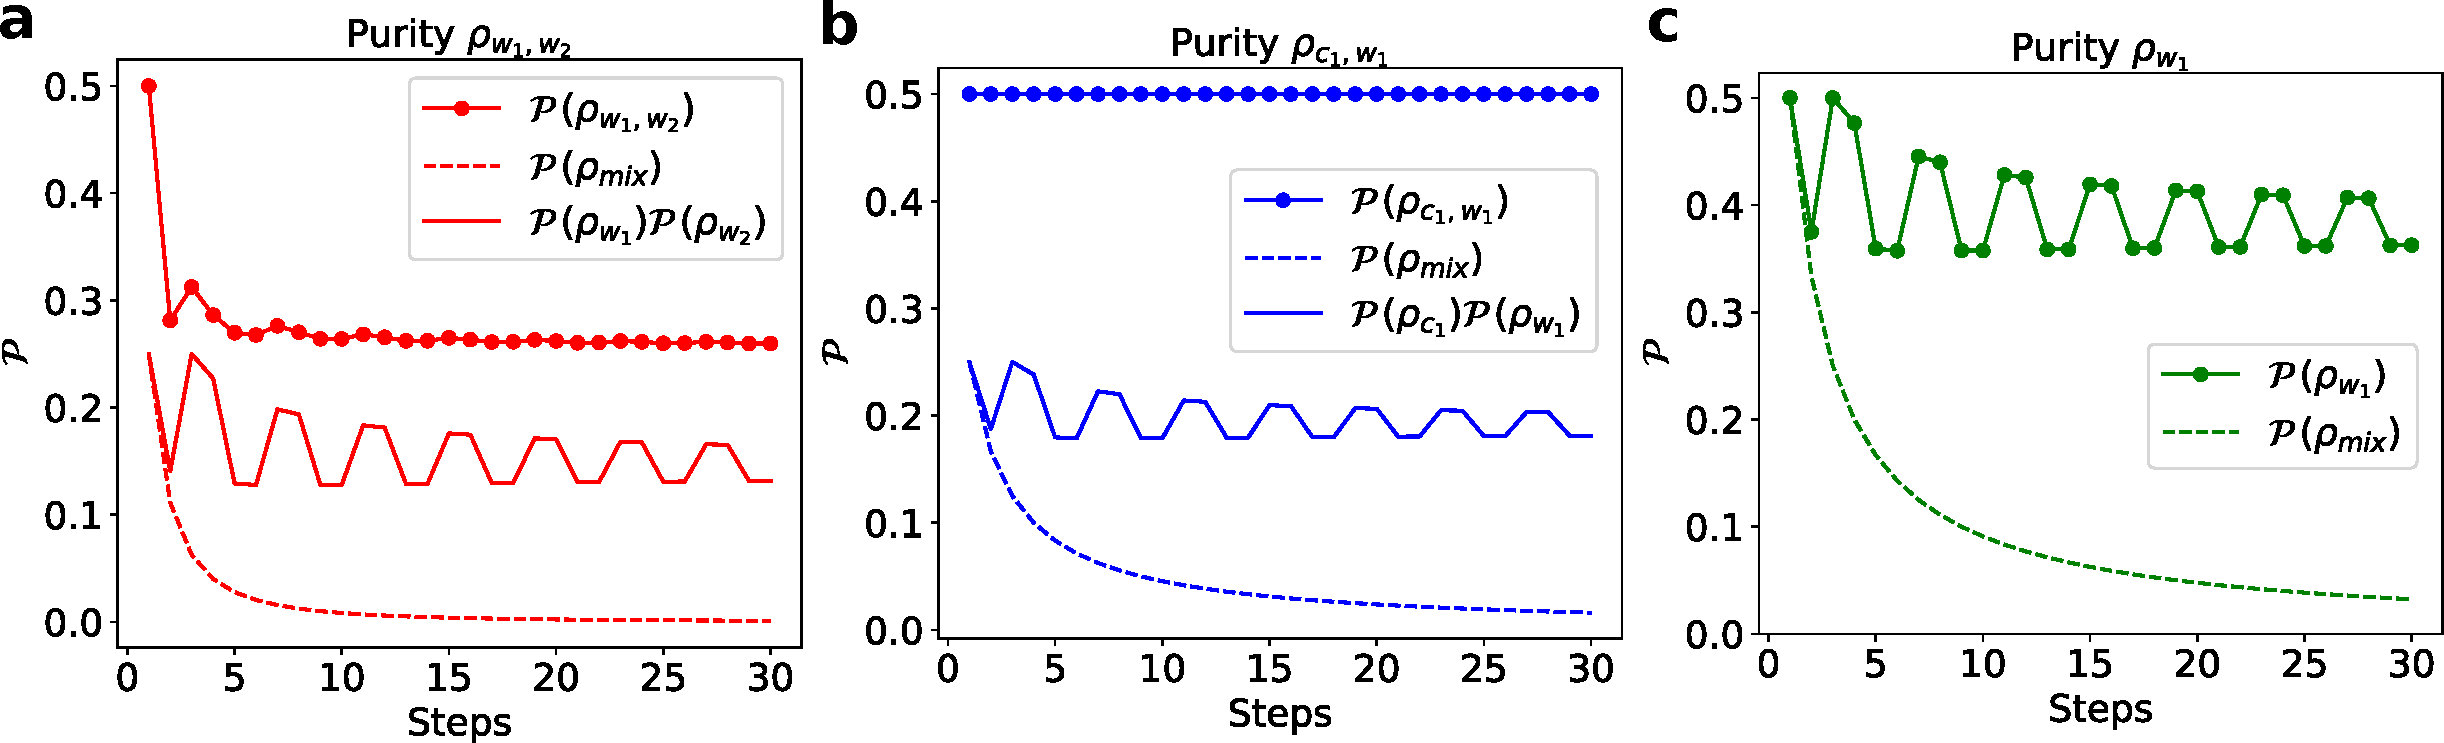
\includegraphics[width=\textwidth]{pur.pdf}
    \caption{\textbf{Purity of traced subsystems}. In each panel we report the purity of the state for different number of steps, of two identical Hadamard quantum walks. The dashed line correspond to the purities of the classical statistical mixture associated to the subspace after investigation.}
    \label{fig:pur_trace}
\end{figure*}
\noindent
 We first consider the properties of resulting states when different subsystem are traced. In \Cref{fig:pur_trace} we report the purities ($\mathcal{P} = \mathrm{Tr}(\rho^2)$) for increasing steps of an Hadamard QW for the following states. Given $\rho^f = \ket{\Psi^f}\bra{\Psi^f}$, we consider the joint walkers state, tracing the polarization $\rho_{w_1,w_2}= \mathrm{Tr}( \rho^f)_{c_1,c_2}$, the state of a single quantum walk tracing the other one $\rho_{c_1,w_1}= \mathrm{Tr}( \rho^f)_{c_2,w_2}$ and the state of a single walker tracing the remaining subsystems $\rho_{w_1}= \mathrm{Tr}( \rho^f)_{c_1,c_2,w_2}$.
 The state purity of the traced subsystem could provide a first insight on the entanglement structure of the state. We consider for simplicity two identical Hadamard quantum walks (the general case will be discussed later). If $\rho_{w_1,w_2}$ can be expressed as $\rho_{w_1}\otimes \rho_{w_2}$, then we would have $\mathcal{P}(\rho_{w_1,w_2}) = \mathcal{P}(\rho_{w_1})\cdot \mathcal{P}(\rho_{w_2})$. In \Cref{fig:pur_trace}a we show that the purity for the subsystem $(w_1, w_2)$ is always greater then the product of purities of single walkers. Same behaviour for $\rho_{c_1,w_1}$ respect with the its corresponding subsystems.
 Such intuition regarding residual correlation existing between the two walkers position on their own lattices, and in between the inner coin and position of one particle, is confirmed by the states negativities reported in \Cref{fig:neg_trace}a.
 
 We then consider the most general cases, namely two different unitaries transformation made by random step-dependent coin operators. In \Cref{fig:neg_trace}b and c we report the histograms the state negativities of $\rho_{w_1,w_2}$ and $\rho_{c_1, w_1}$, associated to samples of $1000$ sets $(U_1,U_2)$ for different number of steps. The histograms seem to become more peacked around higher value of negativities with increasing number of steps.

 
\begin{figure*}[hbt]
    \centering
    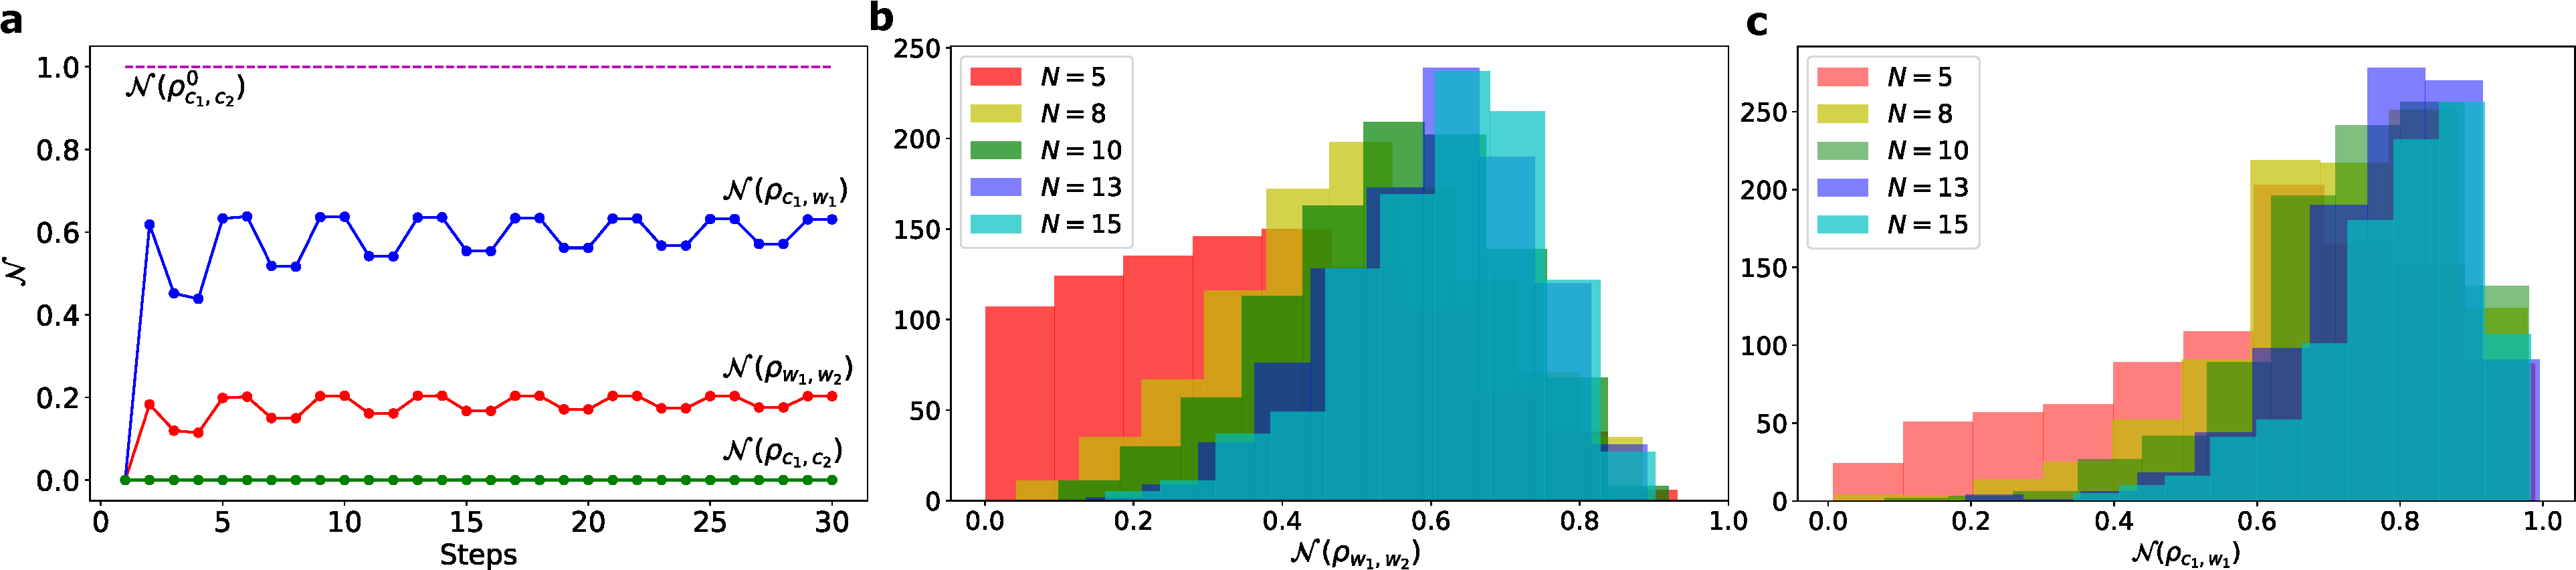
\includegraphics[width=\textwidth]{negs+rand.pdf}
    \caption{\textbf{Negativity criterion}. a) We report the state negativity, for each step of two Hadamard QWs, in different conditions. We consider in red the subsystems associated to the two walkers positions $(w_1,w_2) $ tracing the two coin, in green the system of the two coin tracing the positions $(c_1, c_2)$ and in blue the system of a single quantum walker tracing the other one, namely $(c_1, w_1)$ in the plot. In magenta the negativity of the initial Bell state in the coin degree of freedom. We observe a non-zero negativity between the two walkers. b-c) Histograms of $\rho_{w_1, w_2}$ and $\rho_{c_1, w_1}$ negativities for $1000$ random sampled unitaries. Relaxing the condition of identical QWs and allowing the coin to change at each step, higher values of negativities can be obtained. Furthermore the average increases with the number of step.}
    \label{fig:neg_trace}
\end{figure*}



\section{Projected states}
The previous investigation on the state after trace operation, shows that $\rho_{w_1, w_2}$ has a certain amount degree of entanglement. Now we look for saturating the bound, projecting the coin on suitable directions. First, let us define a generic coin projectors, starting from the orthonormal basis

\begin{align}
 \ket{0} &= \cos{\frac{\theta}{2}} \ket{\uparrow}+ 
 \mathrm{e}^{\mathrm{i}\phi}\sin{\frac{\theta}{2}}\ket{\downarrow} \notag\\
 \ket{1} &= \sin{\frac{\theta}{2}} \ket{\uparrow}-
 \mathrm{e}^{\mathrm{i}\phi}\cos{\frac{\theta}{2}}\ket{\downarrow}
\end{align}

\noindent
where $\theta \in [0, \pi ]$ and $\phi \in [0, 2\pi]$. We then define the four projectors for two separable measurements on the two coin subspace as $\hat{P}_{lm}(\theta, \phi)= \hat{P}_{l}(\theta, \phi)\otimes \hat{P}_{m}(\theta, \phi) = \ket{lm}\bra{lm}$, with $l,m = \{\ket{0}, \ket{1}\}$. After applying these operators on the state in \cref{eq:final_state} we obtain the following states in the $(w_1, w_2)$ subspace
\begin{subequations}
\label{eq:prj_state}
\begin{align}
    \hat{P}_{00} &\rightarrow \alpha_{00}\ket{\psi^{0 \uparrow}_1 \psi^{0 \downarrow}_2} + \beta_{00}\ket{\psi^{0 \downarrow}_1 \psi^{0 \uparrow}_2} \label{eq:prj_state_a}\\
    \hat{P}_{01} &\rightarrow \alpha_{01}\ket{\psi^{0 \uparrow}_1 \psi^{1 \downarrow}_2} + \beta_{01}\ket{\psi^{0 \downarrow}_1 \psi^{1 \uparrow}_2}\label{eq:prj_state_b}\\
    \hat{P}_{10} &\rightarrow \alpha_{10}\ket{\psi^{1 \uparrow}_1 \psi^{0 \downarrow}_2} + \beta_{10}\ket{\psi^{1 \downarrow}_1 \psi^{0 \uparrow}_2}\label{eq:prj_state_c}\\
     \hat{P}_{11} &\rightarrow \alpha_{11}\ket{\psi^{1 \uparrow}_1 \psi^{1 \downarrow}_2} + \beta_{11}\ket{\psi^{1 \downarrow}_1 \psi^{1 \uparrow}_2}\label{eq:prj_state_d}.
\end{align}
\end{subequations}

In the above expression the wavefuctions $\psi^{lk}_i$ are the result of the projection along $l$ of the output state $\ket{\Psi^{k}_i}$, namely the state after the single particle quantum walk $U_i$, with $k$ as initial coin.

\begin{figure*}[t]
    \centering
    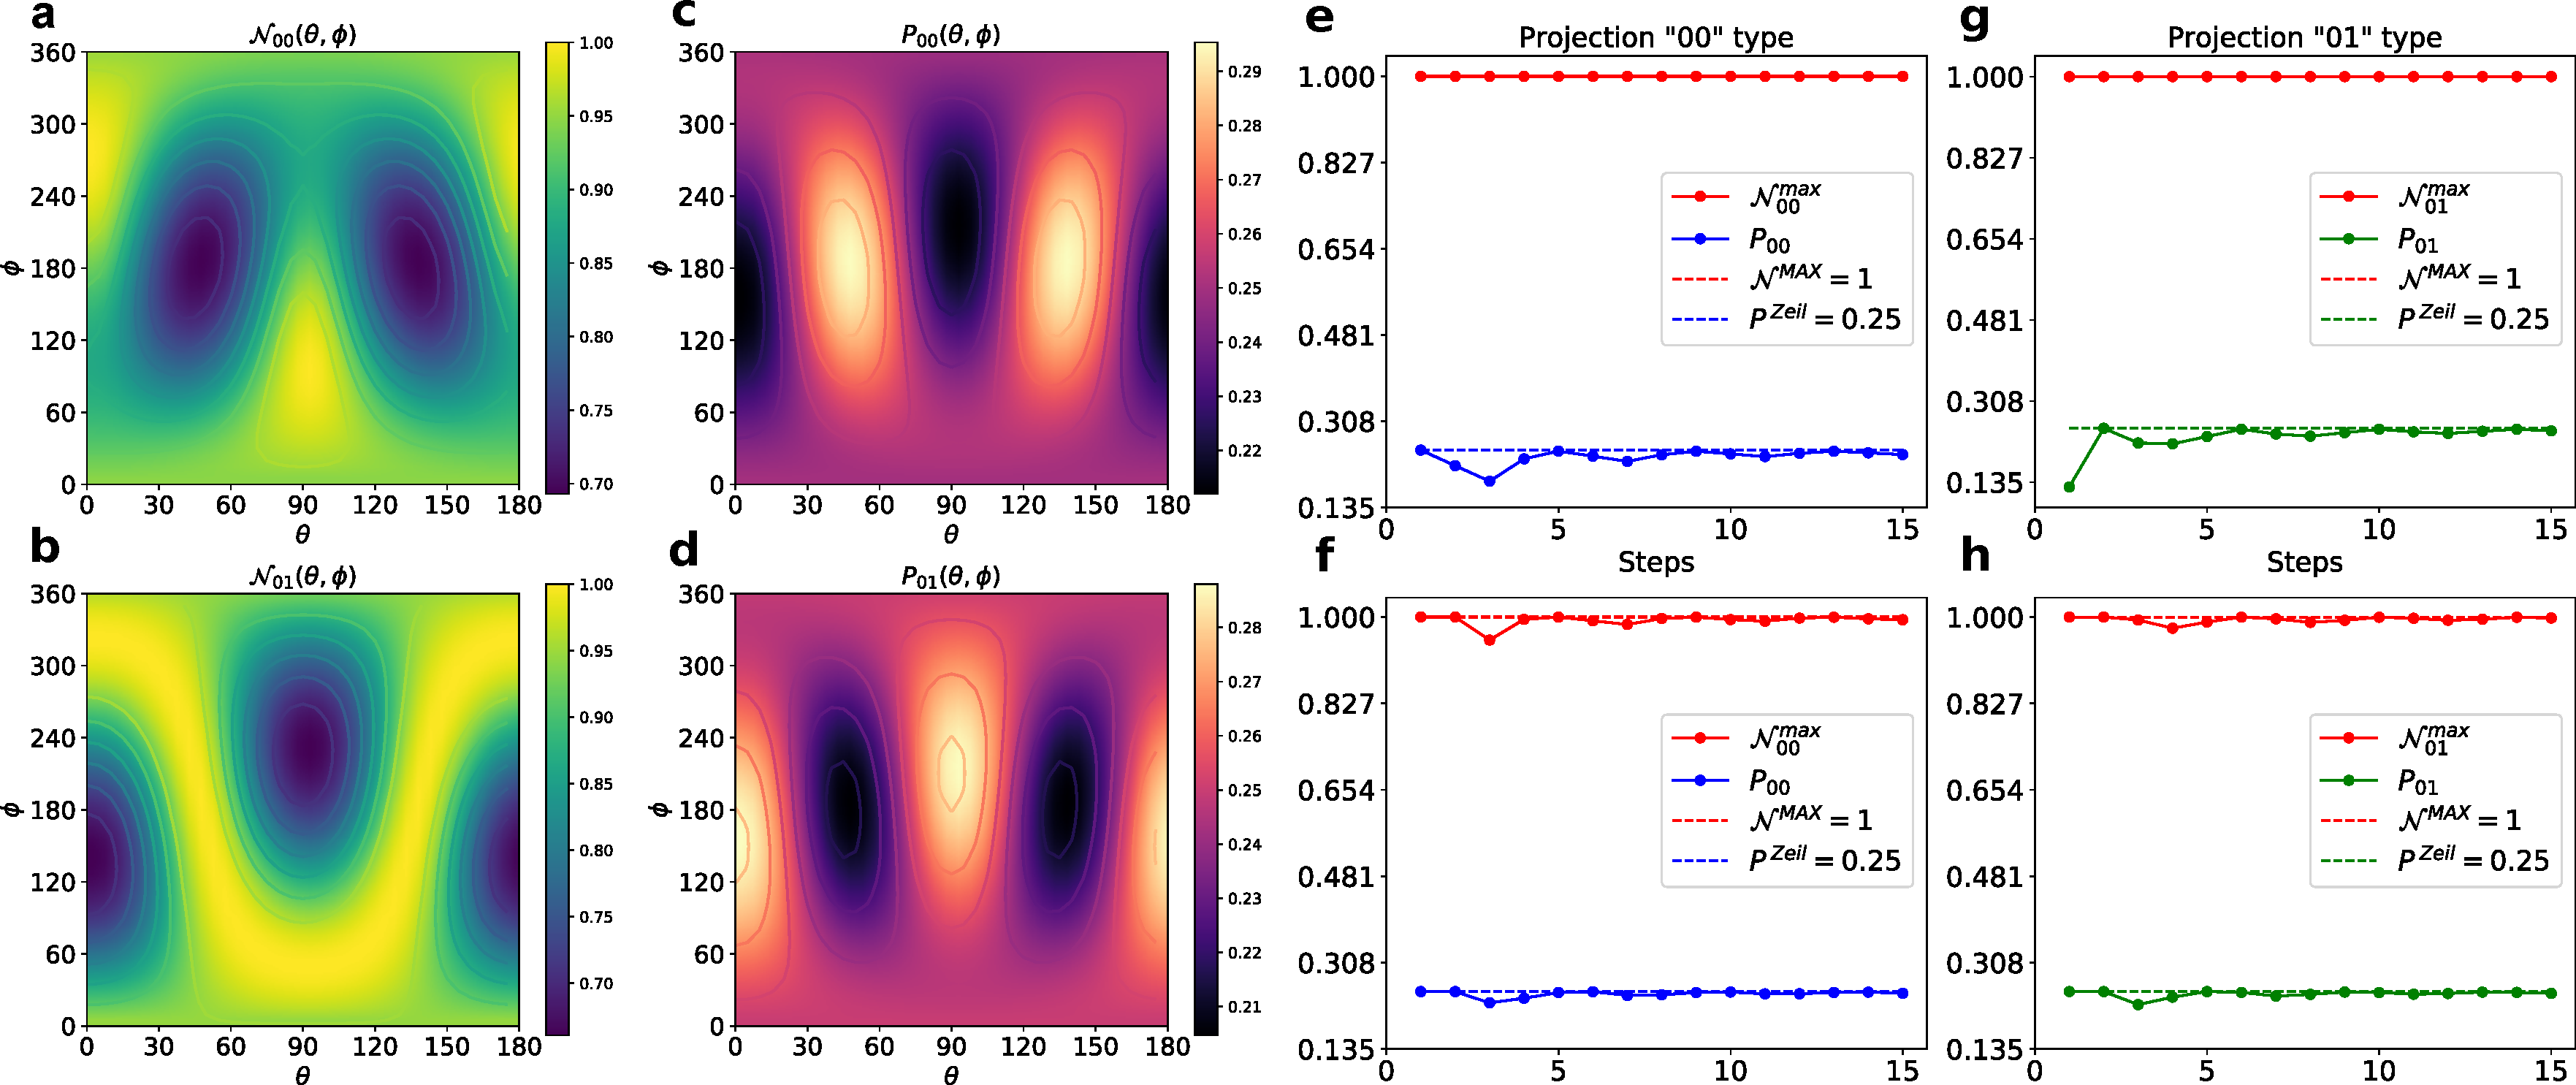
\includegraphics[width=\textwidth]{proj.pdf}
    \caption{\textbf{Projection optimization for Hadamard quantum walks.} a-b) State negativities for different type of projection $00$ and $01$ (the other two cases display the same behaviour)in terms of $(\theta, \phi)$. It is worth to note that $\mathcal{N}_{lm}>0.6$ in both cases. c-d) Corresponding surface for the projection probabilities. It is possible to obtain $P_{lm}> 0.25$ (generation probability of Ref \cite{fickler2012quantum}) but with non-optimal negativity. e-f) $\mathcal{N}_{00}$ and $P_{00}$ respect with different number of steps in the case e) of $\mathcal{N}_{00}$ optimization and f) for the maximization of both $\mathcal{N}_{00}$ and $P_{00}$. We note that both bound ($1, 0.25$) can be saturated by our protocol. g-h) same calculation of panels e-f) for $01$ projection.}
    \label{fig:10steps_results}
\end{figure*}
We firstly investigate, as in the previous section, the case $U_1 = U_2$. The states in \cref{eq:prj_state_a} and  \cref{eq:prj_state_d} can be rewritten as $\alpha \ket{\psi_a \psi_b} + \beta \ket{\psi_b \psi_a}$, since only two type of qudits can be obtained. In literature such state has been already generated exploiting the entanglement of a Bell state in polarization qubits which is transferred to a state in the orbital angular momentum (OAM). In such apparatus the two QW are replaced by two Sagnac-interferometer with one spatial light modulator per part displaying two holograms $\{\psi_a, \psi_b\}$ \cite{fickler2012quantum}. The resulting state is similar to the expression \cref{eq:final_state} but with single particle states in which polarization and OAM are separable, i.e $\ket{\Psi^{Zeil}}=A(\ket{\uparrow \psi_a}\ket{\downarrow \psi_b} +\ket{\downarrow \psi_b} \ket{\uparrow \psi_a})$. Despite the similarities of the two techniques it is worth to that this state cannot display the same properties under coin tracing. Indeed in the case of $\braket{\psi_a}{ \psi_b}=0$, which ensure the maximum negativity when the state is projected with $\hat{P}_{00}(90\degree,0)$, does not display entanglement when the polarization is traced (the state is a statistical mixture of $\{\psi_a, \psi_b\}$). Furthermore if we look at the states of \cref{eq:prj_state_b} and \cref{eq:prj_state_c}, they need in general four type of qudits to be described even with two identical unitaries. These states could be reproduced by the apparatus of Ref. \cite{fickler2012quantum} but with at least four holograms.

We now test the capability of our setup for generating states in \cref{eq:prj_state} with maximum negativity, in the case of two identical Hadamard QWs. We search for a optimal set of $(\theta, \phi)$ parameter that maximize both the negativity and the projection probability. We find two sets that maximize these quantities for the projections types $\{00, 11\}$ and $\{01, 10\}$ respectively. In \Cref{fig:10steps_results}a,b we report the value of negativities and projection probabilities in terms of the two parameters for $N=10$ steps. It is worth to note that exist large areas in which $\mathcal{N}_{lm}$ assumes the value 1. In the panels e-h of \Cref{fig:10steps_results} we report the values of $\mathcal{N}_{lm}$ and $\mathcal{P}_{lm}$ for any step for both set of optimal parameter, when the maximization is performed \textit{i)} on the neagativity and \textit{ii)} both the negativity and projection probabilities. In particular we compare the latter with the generation probability of Ref. \cite{fickler2012quantum}.
Same results can be obtained with random sampled quantum walks: it is always possible to find optimal projectors for retrieving the ebit of entanglement in the two walkers state.

\section{Entanglement accumulation}
\noindent
Here we ask if it could be possible to accumulate more than one ebit of entanglement in the walkers spaces, iterating the two parallel QWs protocol. After the first round and the optimal projection of the coin, the output is one of the states of \cref{eq:prj_state}. Since the coin and walkers position are now separable again, as in the previous input states, one can generated a new Bell state in the coin degree of freedom. Such operation can be performed with an Hadamard gate on the first qubit, followed by C-NOT operation, $U^{Bell} = U_{CNOT}*(H_1 \otimes I_2)$.

Let us consider the case in which for simplicity the first projection is 00 type and the unitaries are identical. The input state for the second iteration, after the $U^{Bell}$ on the coin
 \begin{align}
     \ket{\Psi^{0 (1)}} &= \frac{1}{2}\left(\ket{\uparrow \psi_a}_1 \ket{\uparrow \psi_b}_2 +\ket{\uparrow \psi_b}_1 \ket{\uparrow \psi_a}_2 + \right \notag\\
      &\left + \ket{\downarrow \psi_a}_1 \ket{\downarrow \psi_b}_2 +
     \ket{\downarrow \psi_b}_1 \ket{\downarrow \psi_a}_2
     \right),
 \end{align}
injected to the others QWs, will produce the state
\begin{align}
     \ket{\Psi^{f(1)}}&= \alpha\ket{\Psi^{\uparrow \psi_a}_1\Psi^{\uparrow \psi_b}_2} + \beta
     \ket{\Psi^{\uparrow \psi_b}_1\Psi^{\uparrow \psi_a}_2}+  \notag \\
                     &+ \delta \ket{\Psi^{\downarrow \psi_a}_1\Psi^{\downarrow \psi_b}_2} +\gamma  \ket{\Psi^{\downarrow \psi_b}_1\Psi^{\downarrow \psi_a}_2}.
\label{eq:final_state1}                 
\end{align}

\begin{figure}[t]
\centering
    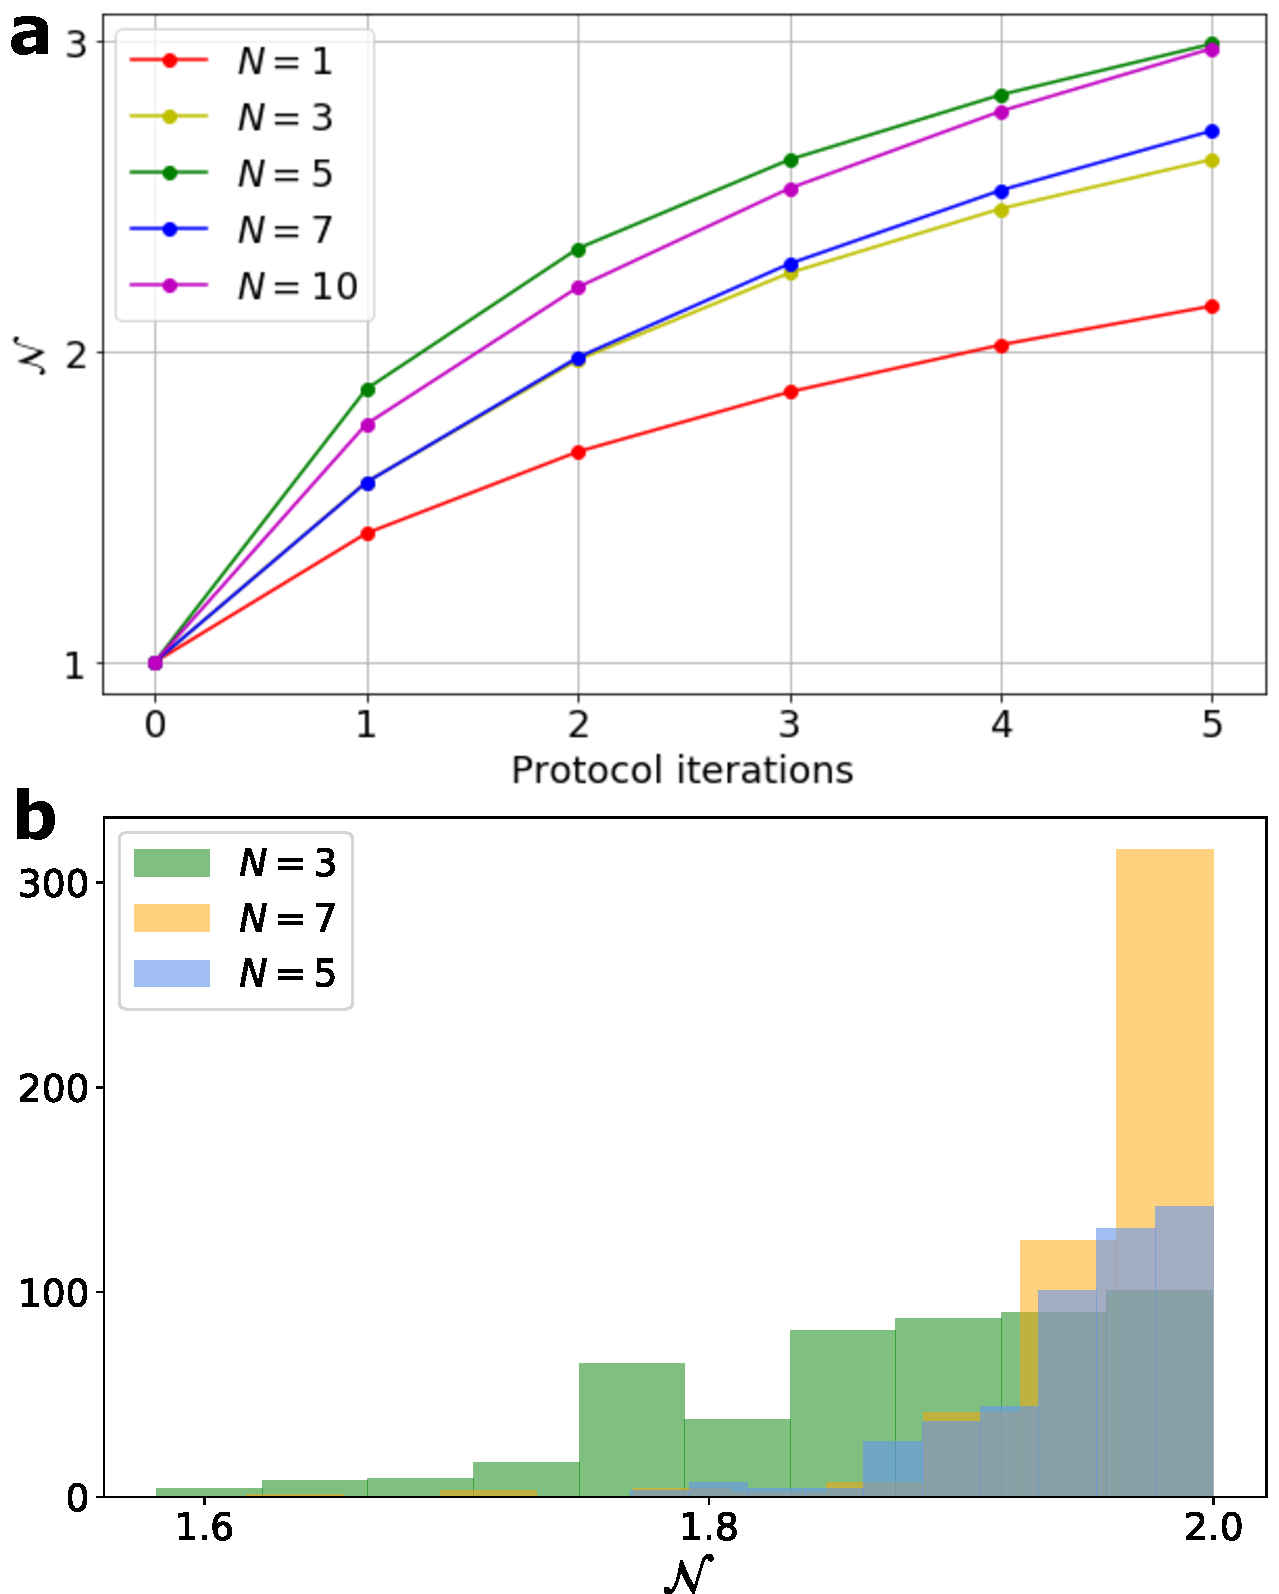
\includegraphics[width = \columnwidth]{figures/scaling.pdf}
    \caption{\textbf{Entanglement accumulation} a) Trend of the entanglement accumulation after several iterations of the protocol with identical Hadamard QW of $N=\{1,3,5,7,10\}$ steps. From such simulation seems that the optimal transfer of one ebit per iteration cannot be reached. However, relaxing the need to have same unitaries at each step, the optimal scaling can be obtained. b) Histograms for one iteration of entanglement transfer protocol (the stage zero with two identical Hadamard QWs), for three values of QW steps per iteration $N=\{3,5,7\}$. 
    Each histograms represent the distribution of $500$ random extracted coin operators for individuating the QW unitary to apply to the two walkers in the state $\ket{\Psi^{0(1)}}$. We observe that it is possible to find unitary operation for the second entanglement transfer which allows to saturate the bound of 2 ebit of entanglement. In particular histograms tend to pick towards 2 with increasing number of steps. All the calculations were performed considering coin projection of type $00$.}
    \label{fig:ent_acc}
\end{figure}
It is clear that after a further coin projection, the whole state will collapse in a superposition of four terms with at least four different qudits states involved.
Due to the high-dimension of the two walkers position, we can generate states in which the four qudits in the superposition are mutually orthogonal. To be more precise,
let us consider, as example, a state $\ket{q} = \sum_{s =1}^{n_q} \ket{ss}$, where $s$ are the walkers position. The negativity of such state scales as $\log_2(n_q + 1)$. According to such intuition we expect that the maximum negativity of the state $\ket{\Psi^{f(N_i)}}$ at the iteration $N_i$ after a proper coin projection, could be $\mathcal{N}^{Max} =\log_2( 2^{N_i}+1)$. Indeed the number of states in the superposition grows as $2^{N_i}$, as can be verified looking at \eqref{eq:final_state} and \eqref{eq:final_state1}.

In Fig. \ref{fig:ent_acc}a we report numerical simulation on the scaling of negativity according to increasing number of iteration. We consider cascaded Hadamard QWs, starting from the initial state in \eqref{eq:initial_state}, with $U^{Bell}$ coin operation in between. We focus on iteration in which the optimization on the negativity is performed on projectors of type $00$, after Qws of equal steps $N$, for different value of $N$. According to this simulation, the optimal curve $\mathcal{N}^{Max}$ is not saturated. For improving the performance of the protocol different strategies can be investigated. In 
Fig. \ref{fig:ent_acc}b we try to change the unitary after the first optimal coin projection on two Hadamard QWs. To this aim 
we have random sampled the coin operators for the next QWs evolution, considering the accumulation after one iteration of the protocol for different steps. From such simulation turns out that there is a dependence both from the choice of the unitary in the second stage and from the number of steps of each QW (see Fig. \ref{fig:ent_acc}b). The latter is not surprising since with high number of steps we cover higher dimensional Hilbert spaces and, consequently, it could be easier to produce four qudits mutually orthogonal inside the state produced by the projection of the coins in $\ket{\Psi^{f(1)}}$.








%It is clear that after a further coin projection, the whole state will collapse in a superposition of four terms with at least four different qudits states involved.
%Due to the high-dimension of the two walkers position, we can generate states in which the four qudits in the superposition are mutually orthogonal (states which display one ebit of entanglement present four qudits entangled too, see previous expression \cref{eq:prj_state}).
%Let us consider a state $\ket{q} = \sum_{s =1}^{n_q} \ket{ss}$, where $s$ are the walkers position. The negativity of such state (normalized to the ebit) scales as $n_q - 1$. According to such intuition we expect that the maximum negativity of the state $\ket{\Psi^{f(N_i)}}$ at the iteration $N_i$ after a proper coin projection, is at least $\mathcal{N}^{Max} = 2^{N_i}-1$. Indeed the number of states in the superposition grows as $2^{N_i}$, as can be verified looking at \cref{eq:final_state} and \cref{eq:final_state1}.

%In \Cref{fig:ent_acc} we report numerical simulation on the scaling of negativity according to increasing number of iteration. We consider cascaded Hadamard QWs, starting from the initial state in \cref{eq:initial_state}, with $U^{Bell}$ coin operation in between. We focus on iteration in which the optimization on the negativity is performed on projectors of type $00$ and $01$, after Qws of equal steps $N$, for different value of $N$. According to this simulation, the optimal curve $\mathcal{N}^{Max}$ is not saturated. For improving the performance of the protocol different strategies can be investigated: using different unitaries at each iteration, projecting on two different single coin measurement, i.e. optimizing on 4 parameters, or varying the number of steps at each iteration.



\subsection{A proof-of-principle experiment}
Here we propose a scheme for the realization of the entanglement accumulation protocol in a photonic platform that encodes coin and walkers position in polarization and OAM degree of freedom. This proposal provides the realization of two iterations, giving access to states with 2 ebit of entanglement. 

The scheme works as follows. It requires that at first iteration the two Qws are identical and to perform type 00 projection on the coins. In this way, the state after the projection that maximize the negativity will be $1/\sqrt{2}\ket{\uparrow \uparrow}\otimes(\ket{\psi_a\psi_b}\pm\ket{\psi_b\psi_a})$. 
It is straightforward to show that the action of a polarizing beam-splitter combined with two half waveplates can perform with probability $1/2$ the $U^{Bell}$ needed to perfom the accumulation.
Indeed, rewriting the state in terms of creation operators we have:
\begin{equation}
    \frac{1}{\sqrt{2}}\left(a^{\dagger}_{\uparrow, \psi_a,1}a^{\dagger}_{\uparrow, \psi_b,2}+a^{\dagger}_{\uparrow, \psi_b,1}a^{\dagger}_{\uparrow, \psi_a,2} \right)\ket{0} 
    \label{eq: snd_quant}
\end{equation}
The two photon are injected in the two input port of a polarizing beam-splitter, after a polarization rotation made by two half-waveplate (see \Cref{fig:exp_ent_acc}). Then creator operators in \cref{eq: snd_quant} become

\begin{align}
    a^{\dagger}_{\uparrow, \psi_{a/b},1} & \rightarrow \cos{\theta_1}a^{\dagger}_{\uparrow, \psi_{a/b},1} + \mathrm{i}\sin{\theta_1}a^{\dagger}_{\downarrow, \psi_{a/b},2}\notag \\
     a^{\dagger}_{\uparrow, \psi_{a/b},2} & \rightarrow \cos{\theta_2}a^{\dagger}_{\uparrow, \psi_{a/b},2} + \mathrm{i}\sin{\theta_2}a^{\dagger}_{\downarrow, \psi_{a/b},1}
\end{align}

\begin{figure}[t]
    \centering
    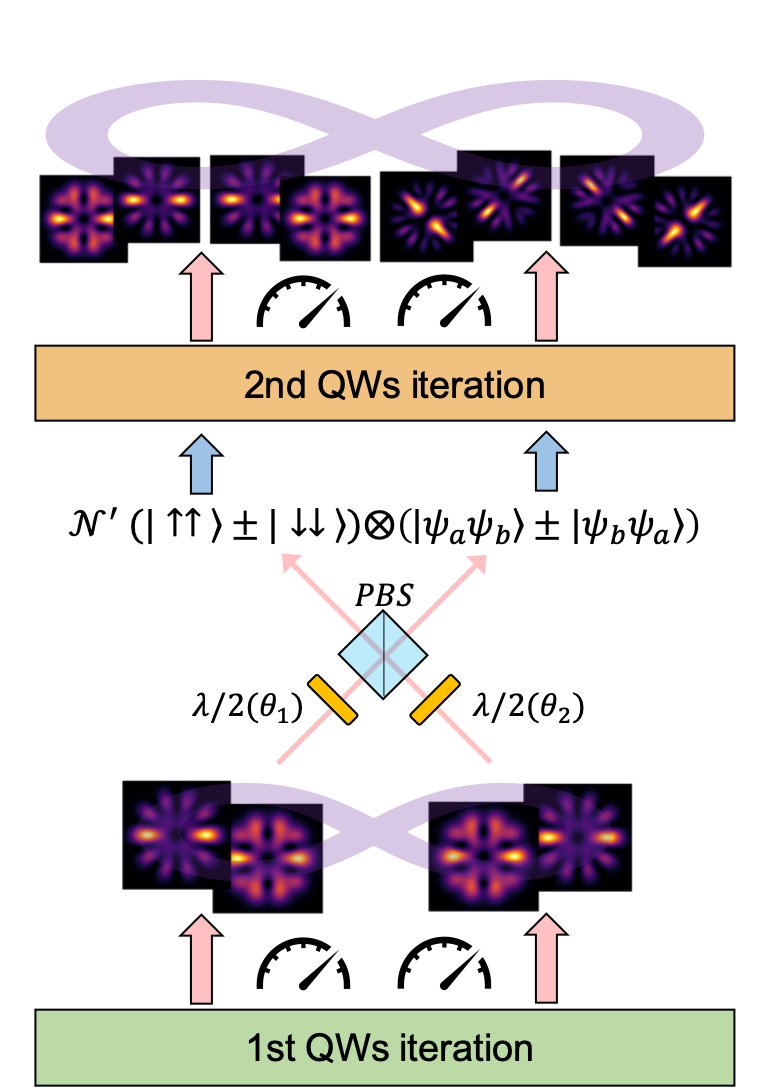
\includegraphics[scale= 0.45]{exp_ent_acc.png}
    \caption{\textbf{Experimental proposal}}
    \label{fig:exp_ent_acc}
\end{figure}


Substituting such expression in \cref{eq: snd_quant} and considering $\theta_1 = \theta_2$ we obtain 
\begin{align}
\frac{1}{2}& * \frac{\left( \ket{\uparrow \uparrow} \pm
\ket{\downarrow \downarrow}\right) }{\sqrt{2}}\otimes \frac{\left( \ket{\psi_a \psi_b} \mp
\ket{\psi_b \psi_a}\right) }{\sqrt{2}} +\notag\\
+\frac{1}{2}& *\frac{\left( \ket{20} +
\ket{02}\right) }{\sqrt{2}}
\end{align}
The first part of the states correspond to resource needed for the protocol accumulation. We can discard the second contribution by post-selecting two fold coincidences between single-photon detectors at the end of second iteration. It is worth to note that the probabilistic generation of the second Bell state is due by the choice to encode qubits in photons. However it is worth to note that we could consider also the state  produced by the projection 11 after the first operation. Indeed it produces, with the same set of optimal $(\theta, \phi)$ parameters, states with the same symmetry properties. In this way it is possible to double the probability of generating states with more than one-ebit of entanglement.

%After a first research in literature, the maximum amount of entanglement generated with %OAM seems to be 3 ebit. In Ref. \cite{Malik2016}, the authors produce 3 entangled %qutrits in a 3-photon experiment.

\section{Entanglement transfer via polarisation projection}
Consider the following scenario: two polarisation-entangled photons evolve independently with the same unitary $\mathcal U$, which entangles their polarisation and OAM degrees of freedom. After the evolution, the polarisations are projected. Is it possible with such a scheme to transfer the polarisation entanglement into the OAMs?

Suppose the two photons are initially the state
\begin{equation}
    \ket{\on{initial}}\equiv
    (a_{p_0,\ell_0,H}^\dagger
    a_{p_1,\ell_0,V}^\dagger +
    a_{p_0,\ell_0,V}^\dagger
    a_{p_1,\ell_0,H}^\dagger) \ket{\mathrm{vac}},
    \label{eq:proj_initial_state}
\end{equation}
for some initial OAM $\ell_0$, and with $p_i, i=0,1$ the $i$-th position.
Note that~\cref{eq:proj_initial_state} is nothing but a state of the form $\ket{HV}+\ket{VH}$ in second quantisation notation.
As long as no operation interfering the two photons is used, we can safely operate in this bra-ket notation.
Evolving the photons locally with the same unitary $\U$ gives
$(\U\otimes\U)(\ket{HV}+\ket{VH})$.
Let us then define
$\ket{\Psi^s}\equiv\U\ket s$, with $s\in\{H,V\}$.
The states $\ket{\Psi^s}$ are one-photon states which in general display entanglement between their polarisation and OAM degrees of freedom:
\begin{equation}
    \ket{\Psi^s}=
    \cos\theta_s \ket H\otimes\ket{\Psi^s_{H}} +
    \sin\theta_s \ket V\otimes\ket{\Psi^s_{V}},
\end{equation}
for some angle $\theta_s$ and states $\ket{\Psi^s_p}$.
Moreover, the unitarity of $\U$ implies that $\braket*{\Psi^H}{\Psi^V}=0$, which translates into the following constraint for $\theta_s$ and $\ket{\Psi^s_p}$:
\begin{equation}
    \cos^2\theta_s\braket*{\Psi^H_H}{\Psi^V_H} +
    \sin^2\theta_s\braket*{\Psi^H_V}{\Psi^V_V} = 0.
\end{equation}
The output state thus reads
\begin{equation}
    \ket{\on{out}}
    % \equiv (\U\otimes \U)(\ket{HV}+\ket{VH})
    = \frac{1}{\sqrt2}\left(
    \ket*{\Psi^H,\Psi^V} + \ket*{\Psi^V,\Psi^H}
    \right).
    \label{eq:proj_output_state}
\end{equation}
The question is now whether we can find polarisation projections $\ket\gamma$ and $\ket\delta$ such that $\braket{\gamma\delta}{\on{out}}$ is maximally entangled between the OAM degrees of freedom.
For ease of notation, let us write the set of amplitudes of $\ket{\Psi^s}$ as $\Psi^s_{i\alpha}$, where $i$ covers the OAM degree of freedom and $\alpha$ the polarisation one.
In this notation, $\ket{\on{out}}$ is characterised by the amplitudes $\Psi_{ij,\alpha\beta}$ satisfying
\begin{equation}
    \sqrt2 \Psi_{ij,\alpha\beta} =
    \Psi^H_{i\alpha} \Psi^V_{j\beta} +
    \Psi^V_{i\alpha} \Psi^H_{j\beta}.
\end{equation}
Projecting onto the polarisation states $\ket\gamma\equiv\gamma_\alpha\ket\alpha$ and $\ket\delta\equiv\delta_\beta\ket\beta$ gives
\begin{equation}
    % \sqrt2\,\gamma_\alpha^*\delta_\beta^* \bs\Psi_{ij,\alpha\beta} =
    \frac{1}{\sqrt2}\Big[
    (\underbrace{
        \gamma_\alpha^*\Psi^H_{i\alpha}
    }_{\psi_i})
    (\underbrace{
        \delta_\beta^*\Psi^V_{j\beta}
    }_{\phi_j}) +
    (\underbrace{
        \gamma_\alpha^*\Psi^V_{i\alpha}
    }_{\psi_i'})
    (\underbrace{
        \delta_\beta^*\Psi^H_{j\beta}
    }_{\phi_j'})
    \Big],
    \label{eq:proj_output_after_proj_indices}
\end{equation}
or $\ket{\psi,\phi}+\ket{\psi',\phi'}$ in bra-ket notation.
To have maximal entanglement it is then sufficient that $\braket{\psi}{\psi'}=\braket{\phi}{\phi'}=0$,
in which case~\cref{eq:proj_output_after_proj_indices} becomes equivalent to a Bell state of the form $\ket{00'}+\ket{11'}$.
The question is thus translated into whether there are coefficients $\gamma_\alpha$ such that
\begin{equation}
    \gamma_\alpha\gamma_\beta^*
    (\Psi^H_{i\alpha}})^* \Psi^V_{i\beta}} = 0.
    \label{eq:proj_suffcondition_for_transfer}
\end{equation}
To see whether this condition can be satisfied by an appropriate choice of projection $\gamma_\alpha$, let us define the vectors $\bs v_k$ as
\begin{equation}
\begin{aligned}
    \bs v_1\equiv \braket*{H}{\Psi^H},\quad
    \bs v_2&\equiv \braket*{V}{\Psi^H}, \\
    \bs v_3\equiv \braket*{H}{\Psi^V},\quad
    \bs v_4&\equiv \braket*{V}{\Psi^V}.
\end{aligned}
\end{equation}

\subsection{New method}
Consider a bipartite state of the form $\ket{HV}+\ket{VH}$.
Applying a local unitary $\calU$ on both sides, we get
$\ket*{\Psi^H,\Psi^V} + \ket*{\Psi^V,\Psi^H}$
for $\ket*{\Psi^H}\equiv \calU \ket H$
and $\ket*{\Psi^V}\equiv \calU \ket V$.
    Suppose that $\ket*{\Psi^s}$ are each embedded into a larger Hilbert space with two internal degrees of freedom (\emph{e.g.} polarisation and OAM), and let us write their amplitudes as $\Psi^s_{\alpha,i}$. We want to figure out whether we can project the first degree of freedom on both sides over some state $\ket\gamma$, and still have a maximally entangled state on the remaining degree of freedom.

Focusing on the first particle, to have a maximally entangled state after the projection, we must have
\begin{equation}
    \langle \langle \gamma, \Psi^H\rangle, \langle \gamma, \Psi^V\rangle\rangle=0,
    \label{eq:orthogonality_condition_to_get_maxent}
\end{equation}
where $\langle \gamma,\Psi^s\rangle$ denotes the state remaining after the projection, that is, the state with amplitudes $\sum_\alpha \bar\gamma_\alpha\Psi^s_{\alpha,i}$.
Explicitly,~\cref{eq:orthogonality_condition_to_get_maxent} reads
$%\begin{equation}
    \sum_{\alpha,\beta,i}
    \gamma_\alpha \bar\gamma_\beta \bar\Psi^H_{\alpha,i} \Psi^V_{\beta,i} = 0.
$ %\end{equation}
Interpreting $(\Psi^s_{\alpha,i})_{\alpha,i}$ as matrices, the problem becomes to find the conditions under which there is a state $\ket\gamma$ such that
\begin{equation}
    \tr[
        (\Psi^H)^\dagger (\gamma\gamma^\dagger) \Psi^V
    ] =
    \mel{\gamma}{\Psi^V(\Psi^H)^\dagger}{\gamma} = 0.
    \label{eq:expval0_condition}
\end{equation}

% Suppose now that $\Psi^H$ and $\Psi^V$ are also each maximally entangled.
% This is a necessary requirement for any such scheme to work.
% In our notation, this is equivalent to them being $2\times N$ rectangular matrices with orthonormal rows.
Let $\bs u_1,\bs u_2$ and $\bs v_1,\bs v_2$ denote the rows of $\Psi^H$ and $\Psi^V$, respectively, and define $C\equiv \Psi^V(\Psi^H)^\dagger$. Then,
\begin{equation}
    C =
    \begin{pmatrix}
        \langle \bs u_1, \bs v_1\rangle & \langle \bs u_2, \bs v_1\rangle \\
        \langle \bs u_1, \bs v_2\rangle & \langle \bs u_2, \bs v_2\rangle
    \end{pmatrix}.
\end{equation}
The orthogonality between $\ket*{\Psi^H}$ and $\ket*{\Psi^V}$ is equivalent to $\tr(C)=0$,
which also implies that $C$ has eigenvalues
$\lambda_\pm = \pm\sqrt{-\det C}$.
Suppose $\det C\neq0$, so that $C$ is ensured to be diagonalisable. In general $C$ is not normal, and thus not \emph{orthogonally} diagonalisable.
If $\ket{\lambda_\pm}$ are the eigenvectors of $C$,~\cref{eq:expval0_condition} is satisfied by
\begin{equation}
    \ket\gamma =
    % \frac{1}{\sqrt{2(1+\Re\langle\bs v_+,\bs v_-\rangle)}}
    % \left(
    % \bs v_+} +
    % e^{i\arg\langle\bs v_+,\bs v_-\rangle} \bs v_-
    % \right).
    \frac{
        % \left(
        \ket{\lambda_+} +
        e^{i\arg\braket*{\lambda_+}{\lambda_-}} \ket{\lambda_-}
        % \right)
    }{
        \sqrt{2(1+\Re\braket*{\lambda_+}{\lambda_-})}
    }.
\end{equation}
We also note that the $\det C\neq0$ condition implies that $\{\bs u_1, \bs u_2\}$ and $\{\bs v_1, \bs v_2\}$ are linearly independent and nonzero: if for example $\{\bs u_1,\bs u_2\}$ is not linearly independent, then $\bs u_2=\alpha \bs u_1$ for some $\alpha\neq0$, which immediately implies $\det C=0$ (and the same argument applies to $\{\bs v_1,\bs v_2\}$).
If $\det C=0$, then there are two possible scenarios. If $C=0$, then it is still diagonalisable, and any $\ket\gamma$ satisfies~\cref{eq:expval0_condition} (albeit different $\ket\gamma$ will correspond to different success probabilities).
For the $C\neq0$ case,
suppose one of the vectors, for example $\bs v_1$, is zero (the other cases proceed similarly). Then we can find a projection $\ket\gamma$ as long as $\on{span}(\{\bs u_1,\bs u_2\})$ contains a vector orthogonal to $\bs v_2$. This is ensured to happen if $\{\bs u_1,\bs u_2\}$ is linearly independent, or if $\langle\bs u_2,\bs v_2\rangle=0$. As an additional condition, we also need $\langle\bs u_1, \bs v_2\rangle\neq0$ if $\langle \bs u_2,\bs v_2\rangle\neq0$.

An example of such scenario is
$\ket*{\Psi^V}=\ket V\ket1$ and
$\ket*{\Psi^H}=\frac{1}{\sqrt2}\left(\ket H\ket2 + \frac{1}{\sqrt2}\ket V(\ket{1} + \ket2)\right)$.
Here, $\bs u_1 = \ket2/\sqrt2$, $\bs u_2=\frac12(\ket1+\ket2)$,
$\bs v_1=0$ and $\bs v_2=\ket1$.
While $\on{span}(\{\bs u_1,\bs u_2\})$ contains $\ket2$, which is orthogonal to $\bs v_2$, we have $\langle \bs u_2,\bs v_2\rangle\neq0$ but $\langle \bs u_1,\bs v_2\rangle=0$, which means that the projection should be $\ket\gamma=\ket H$, which happens with zero probability.

On the other hand, if
$\ket*{\Psi^V}=\ket V\ket1$ and
$\ket*{\Psi^H}=\frac{1}{\sqrt2}\left(\ket H\ket1 + \frac{1}{\sqrt2}\ket V(\ket{1} + \ket2)\right)$,
then the projection $\ket\gamma=\frac{1}{\sqrt3}(-\ket H+ \sqrt2\ket V)$ has nonzero probability and does what we want. 

As an example, suppose
\begin{equation}
\begin{aligned}
    \sqrt2\ket*{\Psi^H} &= \ket H\otimes \ket 1 + \ket V\otimes \ket +, \\
    \sqrt2\ket*{\Psi^V} &= \ket H\otimes \ket - + \ket V\otimes \ket 0.
\end{aligned}
\end{equation}
Then,
$\bs u_1 = \ket 1$, $\bs u_2 = \ket +$,
$\bs v_1 = \ket -$, $\bs v_2 = \ket 0$,
and
\begin{equation}
    C = \begin{pmatrix}
        -\frac1{\sqrt2} & 0 \\
        0 & \frac1{\sqrt2}
    \end{pmatrix}.
\end{equation}
The projection $\ket\gamma=\ket+$ is therefore suitable, as can be directly verified:
% \begin{equation}
% \begin{aligned}
%     \braket*{\gamma}{\Psi^H} &=
%     % \ket1 + \ket+ =
%     \frac{1}{2\sqrt2} \ket0 +
%     \frac12\left(1 + \frac{1}{\sqrt2}\right) \ket1, \\
%     %
%     \braket*{\gamma}{\Psi^V} &=
%     % \ket1 + \ket+ =
%     \frac12\left(1 + \frac{1}{\sqrt2}\right) \ket0
%     - \frac1{2\sqrt2} \ket1.
% \end{aligned}
% \end{equation}
\begin{equation}
\begin{aligned}
    2\sqrt2 \braket*{\gamma}{\Psi^H} &=
    % \ket1 + \ket+ =
    \ket0 +
    \left(\sqrt2 + 1\right) \ket1, \\
    %
    2\sqrt2 \braket*{\gamma}{\Psi^V} &=
    % \ket1 + \ket+ =
    \left(\sqrt2 + 1\right) \ket0
    - \ket1.
\end{aligned}
\end{equation}
% Note how it is not necessary for the internal degrees of freedom on the individual parties to be maximally entangled for this to work.

% The unitarity of $\U$ is then translated into the orthogonality condition $\langle\bs v_1,\bs v_3\rangle+\langle\bs v_2,\bs v_4\rangle=0$, while~\cref{eq:proj_suffcondition_for_transfer} becomes
% \begin{equation}
% \begin{aligned}
%     (\abs{\gamma_H}^2-\abs{\gamma_V}^2) \langle\bs v_1,\bs v_3\rangle &+
%     \gamma_H\gamma_V^* \langle\bs v_1, \bs v_4\rangle \\
%     &+ \gamma_H^*\gamma_V \langle\bs v_2, \bs v_3\rangle = 0.
% \end{aligned}
% \label{eq:proj_conditions_on_vs}
% \end{equation}
% Introducing the angles $\theta,\varphi$ to parametrise the projection $\gamma$, with $\gamma_H=\cos\theta$ and $\gamma_V=\sin\theta e^{i\varphi}$, we get
% % \begin{equation}
% %     \cos(2\theta) \langle\bs v_1,\bs v_3\rangle +
% %     \sin(2\theta)e^{-i\varphi} (
% %         \langle\bs v_1,\bs v_4\rangle +
% %         e^{2i\varphi}\langle\bs v_2,\bs v_3\rangle
% %     ) = 0.
% % \end{equation}
% \begin{equation}
%     \cos(2\theta) +
%     \sin(2\theta) \left[
%         e^{-i\varphi}c_1 +
%         e^{i\varphi}c_2
%     \right] = 0,
%     \label{eq:proj_anglecondition_1}
% \end{equation}
% where we assumed $\langle\bs v_1,\bs v_3\rangle\neq0$, and defined
% $c_1\equiv \frac{\langle\bs v_1,\bs v_4\rangle}{\langle\bs v_1,\bs v_3\rangle}$ and
% $c_2\equiv \frac{\langle\bs v_2,\bs v_3\rangle}{ \langle\bs v_1,\bs v_3\rangle }$.
% On the other hand, if $\langle\bs v_1,\bs v_3\rangle=0$ then~\cref{eq:proj_conditions_on_vs} gives
% \begin{equation}
%     \sin(2\theta)(
%     e^{-i\varphi} \langle\bs v_1,\bs v_4\rangle +
%     e^{i\varphi}\langle\bs v_2,\bs v_3\rangle
%     ) = 0.
%     \label{eq:proj_anglecondition_2}
% \end{equation}
% % which is satisfied if $\theta\in\{0,\pi/2\}$, or $\theta\neq0,\pi/2$ and
% % \begin{equation}
% %     e^{-i\varphi} \langle\bs v_1,\bs v_4\rangle +
% %     e^{i\varphi} \langle\bs v_2,\bs v_3\rangle = 0.
% %     \label{eq:proj_anglecondition_3}
% % \end{equation}
% % In all of these cases, there are angles $\theta,\varphi$ such that the condition is satisfied, implying that one can always find a projection which results in the entanglement being fully transferred into the OAM degree of freedom.
% To see in which cases we can find angles $\theta,\varphi$ satisfying these relations, the crucial observation is that, for any pair of complex numbers $c_1,c_2\in\CC$, the set
% \begin{equation}
%     \{e^{-i\varphi}c_1 +
%         e^{i\varphi}c_2: \varphi\in\RR\}
% \end{equation}
% is an ellipse in $\CC\simeq\RR^2$ centered at the origin.
% It follows that, for all $c_1,c_2\in\CC$, there is some $\varphi\in\mathbb R$ such that $e^{-i\varphi}c_1 + e^{i\varphi}c_2\in\RR$ (indeed, we know that there are exactly two values of $\varphi$ such that this holds).
% Moreover, one of the two axes of the ellipse equals zero (and thus the ellipse collapses to a segment) if and only $\abs{c_1}=\abs{c_2}$ and $\arg c_1+\arg c_2\in\{0,\pi\}$.

% In the case $\langle\bs v_1,\bs v_3\rangle=0$ considered in~\cref{eq:proj_anglecondition_2}, we obtain orthogonal states on the OAM by choosing a projection of the form $\gamma_H \gamma_V=0$, or alternatively if $|\langle\bs v_1,\bs v_4\rangle|=|\langle\bs v_2,\bs v_3\rangle|$ and $\arg \langle\bs v_1,\bs v_4\rangle+\arg \langle\bs v_2,\bs v_3\rangle\in\{0,\pi\}$, via a projection such that $\varphi+\arg \langle\bs v_1,\bs v_4\rangle\in  \pi \ZZ/2$.
% In the more general case with $\langle\bs v_1,\bs v_3\rangle\neq0$,~\cref{eq:proj_anglecondition_1} oughts to be satisfied. Because we can always find $\varphi$ such that $e^{-i\varphi}c_1+e^{i\varphi}c_2\in\RR$, it follows that the condition is equivalent to $\cos(2\theta)+\sin(2\theta)N=0$ for some $N\in\RR$, which is solved by $\theta$ such that $\tan(2\theta)=-1/N$ (unless $N=0$, which happens in the degenerate case in which the ellipse collapses to a vertical segment).

% We conclude that there is always a projection $\ket\gamma$ such that $\braket*{\gamma}{\Psi^H}$ is orthogonal to $\braket*{\gamma}{\Psi^V}$. We can then choose $\ket\delta$ similarly to have $\ket{\on{out}}$, as defined in~\cref{eq:proj_output_state}, become a Bell state embedded in the enlarged OAM state, thus achieving (although probabilistically) perfect entanglement transfer from the polarisation to the OAM.

% The probability of this projection reads
% \begin{equation}
% \begin{aligned}
%     |\braket{\gamma\delta}{\on{out}}|^2 =
%     \frac{1}{2}\big(
%         &\lvert\braket*{\gamma}{\Psi^H}\!
%         \braket*{\delta}{\Psi^V}\rvert^2 \\
%         +
%         &\lvert\braket*{\gamma}{\Psi^V}\!
%         \braket*{\delta}{\Psi^H}\rvert^2
%     \big).
% \end{aligned}
% \end{equation}

\subsection{General setting}

More generally, we can summarise the problem at hand with the following circuit:

\begin{minipage}[c]{\linewidth}
    \centering
    \begin{quantikz}
        \lstick[wires=4]{$\ket{\Psi_{\on{in}}}$}\qw &\qw & \gate[wires=2]{U_{12}}\slice{$\ket{\Psi_f}$} &\qw \\
        % \qw & \gate[wires=2]{U_{23}} & \qw & & \qw & \qw\rstick[wires=2]{$\ket{\Psi_f}$}\\
        \qw & \gate[wires=2]{U_{23}} & & \qw\rstick{$\!\!\!\ket{\gamma}$}\\
        \qw & & \gate[wires=2]{U_{34}} & \qw\rstick{$\!\!\!\ket{\gamma}$}\\
        \qw & \qw & \qw & \qw
    \end{quantikz}
\end{minipage}
The correspondence with the notation used in the previous section is that the first two spaces encode the degrees of freedom of the first photon, third and fourth of the second photon. Second and third spaces correspond to the polarisations of the two photons, and first and fourth spaces to their OAM. It is worth stressing however that the problem studied here goes beyond this particular photonic implementation, and the spaces can have arbitrary dimensions.

The problem we investigate is under what conditions we can find projections $\ket\gamma$ such that the entanglement in $\calH_2\otimes\calH_3$ generated by $U_{23}$ is transferred to $\calH_1\otimes\calH_4$.
Assuming the initial state $\ket{\Psi_{\on{in}}}$ is a product state, the general form of $\ket{\Psi_f}$ reads
\begin{equation}
    \ket{\Psi_f} = \sum_k \sqrt{p_k} \ket{u^k}_{12}\ket{v^k}_{34},
    \label{eq:general_psif}
\end{equation}
where
% $\ket*{u^k}_{12}\in\calH_{12},
% \ket*{v^k}_{34}\in\calH_{34}$, and
$\braket*{u^j}{u^k}=\braket*{v^j}{v^k}=\delta_{jk}$.
This covers all states that can be generated by a circuit of this form for arbitrarily chosen unitaries $U_{12},U_{23},U_{34}$. The entanglement between the subsystems $\calH_{12}$ and $\calH_{34}$ is determined by $U_{23}$, and encoded into the Schmidt coefficients $p_k$ in~\cref{eq:general_psif}.
A point worth stressing is that, if the unitaries $U_{12}$ and $U_{34}$ can be freely chosen, then the problem is trivial. Indeed, one can then trivially fully transfer the entanglement, using for example swap gates (or some similarly defined gates when $\calH_1$ and $\calH_2$ have different dimensions). The setting considered here is thus one in which the gates are assumed to be given.

If we want to optimally transfer the entanglement from $\calH_{23}$ to $\calH_{14}$, we need an output state on $\calH_{14}$ of the form
$\ket*{\Psi_t} = \sum_k \sqrt{p_k}\ket*{\tilde u^k}_1\!\!\ket*{\tilde v_k}_4$.
For this to be the case, we need to find a state $\ket\gamma$ such that the orthogonality is preserved after the projection, that is, such that $\{\!\braket*{\gamma}{u^k}\}_k$ and 
$\{\!\braket*{\gamma}{v^k}\}_k$ are both orthogonal sets.
One way to write this condition is to define the states
$\ket U\equiv\sum_k \ket*{u^k}$
and
$\ket V\equiv\sum_k \ket*{v^k}$,
and ask for a $\ket\gamma$ such that both
$\mel{\gamma}{\PP_U}{\gamma}$
and
$\mel{\gamma}{\PP_V}{\gamma}$
are diagonal with eigenvalues $p_k$,
and $\PP_\psi\equiv\ketbra{\psi}$.
When this is the case, the projection probability is then given by
\begin{equation}
    \det[
        \mel{\gamma}{\PP_U}{\gamma}\mel{\gamma}{\PP_V}{\gamma}
    ].
\end{equation}


\section{Entanglement retrieval (Luca magari \'e gi\'a contenuto nel tuo metodo pi\'u generale?)}

Let us investigate the inverse process for the entanglement transfer, namely from the the state of two entangled walkers to the space of the two coins. Here the question if it is always possible to saturate the maximal amount of entanglement transferable to the space of two qubits. In other word if we can obtain a Bell-like state with one ebit of entanglement via two local identical quantum walks routines and a suitable single-qudit projection in the walker subspace. 

Let's start from the simplest case, an initial state as
\begin{equation}
    \ket{\Psi_0}=\frac{1}{\sqrt{2}}\ket{\uparrow\uparrow}\otimes
    ( \ket{\psi_a\psi_a}+\ket{\psi_b\psi_b})
\end{equation}
in which we require $\braket{\psi_a}{\psi_b}=0$, in order to have one ebit of entanglement at the beginning of the process. Furthermore the dimension $d_0$ of each walkers subsystem is at least two, $d_0\geq 2$. Under the hypothesis of the evolution according to two identical local QWs routine, the final state becomes
\begin{equation}
    \ket{\Psi_f}=\frac{1}{\sqrt{2}}(\ket{\Psi^{\uparrow a}\Psi^{\uparrow a}}+\ket{\Psi^{\uparrow b}\Psi^{\uparrow b}})
    \label{eq:retr1}
\end{equation}
According to the notation of the previous sections, the states $\ket{\Psi^{\uparrow i}}$ are the output of a single-particle QW given as input the coin state $\ket{\uparrow}$ and the walker in $\ket{\psi_i}$. Given the structure of QW's evolution that correlates the two degree of freedoms, the coin and the positions, we can express the $\ket{\Psi^{\uparrow i}}$ as
\begin{align}
    \ket{\Psi^{\uparrow a}}&= a_0\,\ket{0\,\phi_{a_0}} +a_1\,\ket{1\,\phi_{a_1}} \notag\\
    \ket{\Psi^{\uparrow b}}&= b_0\,\ket{0\,\phi_{b_0}} +b_1\,\ket{1\,\phi_{b_1}}
    \label{eq:retr2}
\end{align}
where $\{\ket{0},\ket{1}\}$ is a generic orthonormal basis for the coin subspace and the $\ket{\phi_{i_j}}$ the projections of the state $\ket{\Psi^{\uparrow i}}$ in this basis. 
Now we look for the local qudit projector $\hat{P}_{\phi}=\ketbra{\phi}$ acting on the single subsystem for obtaining a Bell-like state in the two coins. Let us label the overlaps between $\phi$ and single qudit states $\ket{\phi_{i_j}}$ in \eqref{eq:retr2} as
\begin{equation}
    \braket{\phi}{\phi_{i_j}}=\beta_{ij}
\end{equation}
where we remind that index $i=\{a,b\}$ and $j=\{0,1\}$. Then the state after the projection $\hat{P}_{\phi}$ in the two subsystem
\begin{equation}
\begin{split}
    \braket{\phi}{\Psi_f}&=\frac{1}{\sqrt{2}}[(a_0a_1\beta_{a0}\beta_{a1}
    + b_0b_1 \beta_{b0}\beta_{b1})(\ket{01}+\ket{10})+\\
    &+(a_0^2\beta_{a0}^2+b_0^2\beta_{b0}^2)\ket{00}+ (a_1^2\beta_{a1}^2+b_1^2\beta_{b1}^2)\ket{11}]
\end{split}
\end{equation}
Let us observe that a Bell-like state in the form $\frac{1}{\sqrt{2}}(\ket{00}+\ket{11})$ by requiring for example that 
\begin{align}
\beta_{a0}&=\beta_{b1}=0 \\
\frac{b_0}{a_1}&= e^{i \alpha} \frac{\beta_{a1}}{\beta_{b_0}}
\end{align}
\section{Open questions}
\begin{itemize}
    %\item Beyond the ebit: entanglement %accumulation. Iterating the protocol after %a nonlocal operation between the two %parties. Concerning the issue of generating %qudit states in the OAM with more than one %ebit of entanglement, in literature we %found for the moment only this work Ref. %\cite{Malik2016} (3 entangled qutrit). \\
    \item Entanglement retrieval in the polarization. Is it possible to transfer back the ebit to the polarization?
    \item Entangled qudit engineering: given a maximum negativity state, how find the set of unitaries and projections for generating it. To solve this task we have to find
    \begin{itemize}
        \item analytical expression for $\alpha(\beta)_{lm}(\theta, \phi)$
        \item properties of qudits amplitudes in the lattice position basis
    \end{itemize}
    \item Map engineering/inference. How much information about the OAM state of one party can be retrieved from polarization measurements on the other? In this scheme one of the unitaries is the identity.
\end{itemize}

\bibliography{vvb}
\bibliographystyle{apsrev4-1}
\end{document}
